\documentclass[11pt]{article}

%\pagestyle{headings}

\textwidth=440pt
\hoffset=-0.6truein

\usepackage{amsmath}
\usepackage{amsfonts}
\usepackage{amssymb}
\usepackage{authblk}
\usepackage{dsfont}
\usepackage{pifont}
\usepackage{booktabs}
\usepackage{tabularx}
\usepackage{siunitx}
%\usepackage{bbold}
\usepackage{graphicx}
\usepackage{epstopdf}
\usepackage{epsfig}
%\usepackage{bibunits}
%\usepackage{theorem}
%\usepackage[framed]{ntheorem}
\usepackage{framed}
%\usepackage{showlabels}
\usepackage{makeidx}
\usepackage{simplewick}
%\usepackage{tikz-feynman}
\usepackage{hyperref}
\usepackage{placeins}
\usepackage{bbold}
\usepackage[font=small,labelfont=bf]{caption}
%\tikzfeynmanset{compat=1.0.0}
\usepackage{tikz}
\usepackage{braket}
\usetikzlibrary{positioning}% To get more advances positioning options
\usetikzlibrary{arrows}
\usetikzlibrary{colorbrewer}

% barn deprecated by siunitx
\DeclareSIUnit{\barn}{b}

% General global commands
%\newcommand{\cov}{C}
\newcommand{\posterior}[1]{\tilde{#1}}
\newcommand{\real}{\mathbb{R}}
\newcommand{\textin}{\text{in}} 

% General inverse Problems
% map operators
\newcommand{\fwdmapop}{G}
\newcommand{\obsop}{O}
\newcommand{\fwdobsop}{\mathcal{\fwdmapop}}
% model space
\newcommand{\nmodel}{N_{\rm model}}
\newcommand{\modelspace}{X}
\newcommand{\modelvec}{u}
\newcommand{\modelpriorcent}{\modelvec_0}
\newcommand{\modelpriorcov}{\cov_X}
\newcommand{\modelpostcent}{\posterior{\modelvec}}
\newcommand{\modelpostcov}{\posterior{\cov}_X}
% observable space
\newcommand{\ndata}{N_{\rm data}}
\newcommand{\obs}{y}
\newcommand{\obspriorcent}{\obs_0}
\newcommand{\obspriorcov}{\cov_{Y}}
\newcommand{\obsnoise}{\eta}
\newcommand{\obspostcent}{\posterior{\obs}}
\newcommand{\obspostcov}{\posterior{\cov}_Y}
% linear map
\newcommand{\linmap}{\fwdobsop}
\newcommand{\vander}{\mathcal{X}}
\newcommand{\nlaw}{N_{\rm law}}

% NNPDF data/model
\newcommand{\law}{f}
\newcommand{\pseudodat}{\mu}
\newcommand{\noise}{\epsilon}
\newcommand{\repind}{(k)}
\newcommand{\modelvecrep}{\modelvec_*^{\repind}}
% likelihood
\newcommand{\likelihood}{\mathcal{L}}
\newcommand{\repchis}{{\chi^2}^{\repind}}

% closure fitting
\newcommand{\lawmodel}{w}
\newcommand{\utrue}{u_\mathrm{true}}
\newcommand{\uest}{u_\mathrm{est}}

% closure estimators
\newcommand{\testset}[1]{ {{#1}^{\prime}} }
\newcommand{\emodel}[1]{ \mathbf{E}_{\{ \modelvec_* \}} \left[ #1 \right] }
\newcommand{\eout}{\mathcal{E}^{\rm out}}

\newcommand{\nfits}{N_{\rm fits}}
\newcommand{\nreps}{N_{\rm rep}}

\newcommand{\bias}{{\rm bias}}
\newcommand{\var}{{\rm variance}}
\newcommand{\covrep}{\testset{\cov}^{(\rm replica)}}
\newcommand{\covcent}{\testset{\cov}^{(\rm central)}}
\newcommand{\biasvarratio}{\mathcal{R}_{bv}}

% quantile estimators
\newcommand{\xisigdat}[1]{\xi^{(\rm data)}_{#1 \testset{\sigma}}}
\newcommand{\xisigdati}[1]{\xi^{(\rm data)}_{#1 {\testset{\sigma}_i}}}
\newcommand{\modelstd}{\hat{\sigma}}
\newcommand{\erf}{{\rm erf}}

% abbreviations
\newcommand{\ie}{{\it i.e.}}
\newcommand{\eg}{{\it e.g.}}
\newcommand{\viz}{{\it viz.}}

% delta chi2 appendix
\newcommand{\ein}{\mathcal{E}^{\rm in}}
\newcommand{\deltachi}{\Delta_{\chi^2}}
\newcommand{\noisecross}{{\rm noise \, cross \, term}}

% -------------------%
% deprecated commands
% -------------------%
\newcommand{\vv}[1]{\mathbf{#1}}

\newcommand{\vecdiffreptwo}{\left( \vv{\model}^{\repind} - \vv{\levtwo}^{\repind}  \right)}
\newcommand{\vecdiffcentone}{\left( \erep{\vv{\model}} - \vv{\levone} \right)}

\newcommand{\coveig}{\sigma^{2}}
\newcommand{\diag}[1]{\hat{#1}}

\newcommand{\levelonediff}{\Delta}
\newcommand{\underlyingdiff}{u}
\newcommand{\repdiff}{v}

\newcommand{\shiftcross}{{\rm shift \, cross \, term}}
\newcommand{\deltaeps}{\Delta_{\epsilon}}
\newcommand{\kldiv}{D_{KL}}

\newcommand{\diffreptwo}{\left( \model^{\repind} - \levtwo^{\repind} \right)}
\newcommand{\diffcentone}{\left( \erep{\model} - \levone \right)}
\newcommand{\diffcentunder}{\left( \erep{\model} - \law \right)}
\newcommand{\diffcentrep}{\left( \erep{\model} - \model^{\repind}\right)}

\newcommand{\invcov}[1]{\cov^{-1}_{#1}}
\newcommand{\erep}[1]{\mathbf{E}_{\noise}\left[ #1 \right]}
\newcommand{\eshift}[1]{\mathbf{E}_{\shift}\left[ #1 \right]}

\newcommand{\model}{\fwdobsop}
\newcommand{\shift}{\obsnoise}
\newcommand{\invcovprime}{C_D^{\prime -1}}
\newcommand{\levone}{z}
\newcommand{\levtwo}{y}

\newcommand{\npoints}{N_{\rm points}}
\newcommand{\nfit}{\texttt{n3fit}}

\newcommand{\ndat}{N_{\mathrm{dat}}}
\newcommand{\ngrid}{N_{\mathrm{grid}}}
\newcommand{\nflav}{N_{f}}
\newcommand{\NThetaPar}{N_{\Theta\parallel}}
\newcommand{\NThetaPerp}{N_{\Theta\perp}}   
%\newcommand{\nmodel}{N_{\mathrm{model}}}
\newcommand{\cov}{\mathrm{Cov}}
\newcommand{\FKtab}{(\mathrm{FK})}
\newcommand{\FKtabT}{(\mathrm{FK})^T}
\newcommand{\GP}{\mathcal{GP}}
\newcommand{\lat}{{\mathrm{lat}}}
\newcommand{\lin}{{\mathrm{lin}}}
\newcommand{\PDF}{\textrm{PDF}}
\newcommand{\B}{\mathcal{B}} % Basis
\newcommand{\RPDF}{\mathbb{R}^{\PDF}}
\newcommand{\RRPDF}{\mathbb{R}^{\PDF \times \PDF}}
\newcommand{\ddt}{\frac{d}{dt}}
\newcommand{\fin}{f^{\rm in}}

% Matrix
\newcommand{\bpmat}{\begin{pmatrix}}
\newcommand{\epmat}{\end{pmatrix}}

\graphicspath{{./figs/}}

\title{Notes on Neural Tangent Kernels}
\author{Luigi Del Debbio}
\author{Amedeo Chiefa}
\affil{Higgs Centre for Theoretical Physics, School of Physics and Astronomy,
Peter~Guthrie~Tait~Road, Edinburgh EH9 3 FD, United Kingdom.}

\date{\today}
\makeindex

\begin{document}

\maketitle

\begin{abstract}
    Summary of results for NTKs. These notes follow the notation 
    introduced in Ref.~\cite{DBLP:journals/corr/abs-1806-07572}.
\end{abstract}

\section{Definitions}
\label{sec:defs}

\subsection{Neural Networks}
\label{sec:NNDef}

We consider the case of neural networks (NNs) with $L+1$ layers, labelled by the
index $\ell=0,\ldots,L$. The number of neurons in layer $\ell$ is denoted by
$n_{\ell}$. The $\ell=0$ and $\ell=L$ layers are the input and output layers
respectively, so that a NN parametrizes an element of 
\begin{align}
    \label{eq:SetF}
    \mathcal{F} = \left\{ 
        f: \mathbb{R}^{n_0} \to \mathbb{R}^{n_L}
    \right\}\, .
\end{align}
The space of inputs in this case is $\mathcal{X}=\mathbb{R}^{n_0}$, while the
space of outputs is $\mathcal{Y}=\mathbb{R}^{n_L}$. The number of parameters
used in the parametrization is the total number of weights and biases,
\begin{align}
    \label{eq:NumOfPars}
    P = \sum_{\ell=0}^{L-1} (n_\ell + 1) n_{\ell+1}\, .
\end{align}
The weights connecting the layer $\ell$ to the layer $\ell+1$ are denoted
$W^{(\ell+1)}$ and the biases in layer $\ell+1$ are denoted $b^{(\ell+1)}$. 
With this convention
\begin{align}
    W^{(\ell+1)} \in \mathbb{R}^{n_{\ell+1}\times n_{\ell}}\, ,
    \quad 
    b^{(\ell+1)} \in \mathbb{R}^{\ell+1}\, .
\end{align}
When referring to the whole set of parameters, we use the symbol 
\begin{align}
    \theta = \left\{
        W^{(\ell)}, b^{(\ell)}; \; \ell=0, \ldots, L-1
    \right\}\, , 
\end{align}
while individual parameters are denoted $\theta_\mu$, with $\mu=1, \ldots, P$.

The input space is
$\mathcal{X}=\mathbb{R}^{n_0}$ and we consider a probability distribution
$p^{\textin}$ over $\mathcal{X}$, which induces a scalar product in
$\mathcal{F}$,
\begin{align}
    \label{eq:ScalProdX}
    \langle f, g\rangle_{\textin} &= 
        \mathbb{E}_{x\sim p^{\textin}} \left[f(x)^T g(x)\right] \\
        &= \int dx\, p^{\textin}(x) f_i(x) g_i(x)\, .
\end{align}
For a discrete set of datapoints $\mathcal{D}$, 
\begin{align}
    p^{\textin}(x) = \frac{1}{|\mathcal{D}|} \sum_{\alpha\in\mathcal{D}} 
        \delta(x-x_{\alpha})\, ,
\end{align}
where the index $\alpha$ labels the elements of the dataset. For a given set of
parameters, the function parametrized by the NN, which we denote $f_{\theta}$, is given by the
preactivation function of the output layer $L$,
\begin{align}
    f(x;\theta) = \phi^{(L)}(x)\, .
\end{align}
The preactivations $\phi^{(\ell)}$ and the activations $\rho^{(\ell)}$ are
defined recursively as
\begin{align}
    \rho^{(0)}_i(x) 
        &= x_i\, , \\
    \phi^{(\ell+1)}_i(x)
        &= \sum_{j=1}^{n_\ell} W^{(\ell+1)}_{ij} \rho^{(\ell)}_j(x) + b^{(\ell+1)}_i\, , \\
    \rho^{(\ell)}_i(x)
        &= \rho\bigl(\phi^{\ell}_i(x)\bigr)\, ,
\end{align}
where $\rho$ is the activation function. The function 
\begin{align}
    F^{(L)} 
        :\quad & \mathbb{R}^P \to \mathcal{F} \\
        & \theta \mapsto F^{(L)}(\theta) = f_{\theta}
\end{align}
is called the NN realization function. We also introduce the (dual) space of
linear functionals acting on $\mathcal{F }$,
\begin{align}
    \label{eq:FdualDef}
    \mathcal{F}^* = 
        \left\{
            \mu: \mathcal{F} \to \mathbb{R}\,; \; 
                \mu = \langle d, \cdot\rangle_{\textin}, \; d \in \mathcal{F}
        \right\}\, ,
\end{align}
and a loss function 
\begin{align}
    \label{eq:LossDef}
    \mathcal{L}\, : \mathcal{F}\times \mathcal{Z} \to \mathbb{R}\, .
\end{align}
Here $\mathcal{Z}$ denotes the space of datapoints, which we can identify for
now with $\mathcal{X}\times\mathcal{Y}$. 

% The cost function for a set of
% datapoints $\mathcal{D}$ is defined as 
% \begin{align}
%     \label{eq:CostDef}
%     C_{\mathcal{D}}(f) = \frac{1}{|\mathcal{D}|} \sum_{\alpha\in\mathcal{D}}
%     \mathcal{L}(f,z_{\alpha})\, .
% \end{align}

\subsection{Kernel Gradient}
\label{sec:KernGradDef}

A kernel $K$ is defined as a symmetric function 
\begin{align}
    \label{eq:KernDef}
    K: \mathbb{R}^{n_0} \times \mathbb{R}^{n_0} \to 
    \mathbb{R}^{n_L\times n_L}\, ,
\end{align}
such that $K(x,x')=K(x',x)^T$. Using the kernel, a bilinear map is defined 
on $\mathcal{F}$
\begin{align}
    \label{eq:KMap}
    \langle f,g\rangle_K = \mathbb{E}_{x,x'\sim p^{\textin}}
    \left[
        f(x)^T K(x,x') g(x')
    \right]\, .
\end{align}
The kernel is positive definite if
\begin{align}
    ||f||_{p^{\textin}} > 0 
    \quad \Longrightarrow \quad
    ||f||_K > 0\, .
\end{align}
Given a kernel $K$, we define a map
\begin{align}
    \label{eq:PhiKMap}
    \Phi_K: \mathcal{F}^* &\to \mathcal{F} \\
            \mu &\mapsto f_{\mu}\, ,
\end{align}
such that 
\begin{align}
    f_{\mu,i}(x) 
        &= \langle d, K_{i\cdot}(x,\cdot) \rangle_{p^{\textin}} \\
        &= \sum_{j=1}^{n_L} \int dx'\, p^{\textin}(x')\, d_j(x')
            K_{ij}(x,x')\, ,
\end{align}
where $d\in\mathcal{F}$, and $\mu=\langle d, \cdot\rangle_{p^{\textin}}$.

The cost function for a given dataset depends on the values of the function 
$f$ at the datapoints $x_{\alpha}$, so that we can write
\begin{align}
    C_{\mathcal{D}}(f) = \widehat{C}(\mathbf{f})\, ,
\end{align}
where $\mathbf{f}$ is the finite-dimensional vector made of the 
values $f_{\alpha}=f(x_{\alpha})$ for $\alpha=1, \ldots, |\mathcal{D}|$.
The variation of the cost function at a point $f_0 \in \mathcal{F}$ is
\begin{align}
    \left. \delta C_{\mathcal{D}} \right|_{f_0} 
        &= C_{\mathcal{D}}(f_0+\delta f) - C_{\mathcal{D}}(f_0) \\
        &= \sum_{\alpha\in\mathcal{D}} 
            \left. \frac{\partial \widehat{C}}{\partial f_\alpha} \right|_{f_0} 
            \delta f_{\alpha} \\
        &= \left. \partial^{\textin}_{f} C \right|_{f_0} \delta f \\
        &= \langle \left. d\right|_{f_0}, \delta f\rangle_{p^{\textin}}\, ,
\end{align}
where $\delta f \in \mathcal{F}$, $\delta f_{\alpha}=\delta f(x_{\alpha})$ and 
$\displaystyle \left. \partial^{\textin}_{f} C \right|_{f_0} \in \mathcal{F}^*$.

Using the kernel $K$, the {\em kernel gradient} $\left.\nabla_K C\right|_{f_0}$
is defined as 
$\displaystyle \Phi_K\left(\left. \partial^{\textin}_{f} C \right|_{f_0}
\right)$, \ie 
\begin{align}
    \label{eq:KernGradC}
    \left.\nabla_K C\right|_{f_0}(x)
        &= \frac{1}{|\mathcal{D}|} \sum_{\alpha\in\mathcal{D}} 
            K(x,x_{\alpha}) \left. 
            \frac{\partial \widehat{C}}{\partial f_\alpha}\right|_{f_0}\, .
\end{align}
A function $f(t)$ follows the kernel gradient descent if 
\begin{align}
    \partial_{t} f(t) = -\left.\nabla_{K} C\right|_{f(t)}\,.
\end{align}
During the kernel descent, the cost function variation is given by
\begin{align}
    \partial_{t} \left. C\right|_{f(t)}
        &= - \langle \left. d \right|_{f(t)}, \left.\nabla_{K} C\right|_{f(t)} \rangle_{p^{\textin}} = 
        -|| \left. d \right|_{f(t)} ||^2_{K}\, .
\end{align}
More generally, for a function $\widehat{O}$ that depends on 
the values of $f$ on the points in the dataset, 
\begin{align}
    \partial_{t} \left. \widehat{O}\right|_{f(t)}
        &= - \left\langle 
            \frac{\partial \widehat{O}}{\partial f}, 
            \frac{\partial \widehat{C}}{\partial f} 
            \right\rangle_K\, .
\end{align}

\section{Gradient Descent for NNPDF}
\label{sec:GradDescNNPDF}

We work in a basis where the data covariance $C_Y$ is diagonal. Such a choice has two main advantages:
\begin{enumerate}
    \item The data points in this basis are statistically independent, so that when the data is split, 
    e.g. between training and validation sets, the points in each subset are not correlated. 
    \item Working in a basis where the data covariance is diagonal, requires to compute the eigenvectors
    and eigenvalues of $C_Y$, thereby automatically checking for a potentially large condition number. 
\end{enumerate}
Note that, in case we need to apply kinematic cuts, these can be applied before rotating to the diagonal basis. The diagonal basis is then defined by determining the eigensystem of the reduced covariance matrix, i.e. the matrix obtained by removing the lines and columns that correspond to data points that do not pass the kinematic cuts.  

The loss function is defined to be the Mean Square Error (MSE),
\begin{align}
    \label{eq:MSELoss}
    \mathcal{L} &= \frac12 \left(y - T\right)^T C_Y^{-1} \left(y - T\right)\, , \\
        &= \frac12 ||y-T||^2_{C_Y}\, ,
\end{align}
where 
\begin{align}
    \label{eq:DataAndTheory}
    y = 
        \begin{pmatrix}
            y_1 \\
            \vdots \\
            y_I \\
            \vdots \\
            y_{\ndat}
        \end{pmatrix}\, , 
    \quad \mathrm{and} \quad 
    T = 
        \begin{pmatrix}
            T_1 \\
            \vdots \\
            T_I \\
            \vdots \\
            T_{\ndat}
        \end{pmatrix}\, 
\end{align}
are vectors containing the data points $y_I$ and their respective theoretical predictions $T_I$, where $I=1, \dots, \ndat$. The loss function can be written using explicit indices, 
\begin{align}
    \label{eq:MSELossWithIndices}
    \mathcal{L} = \frac12 \sum_I \frac{1}{\sigma_I^2} \left(y_I - T_I\right)^2\, .
\end{align}
However, here and in what follows, we try to minimize the usage of explicit indices.

Denoting by $t$ the training time, and by $\theta_\mu$, with $\mu=1, \dots, P$, the parameters used to specify 
the functional form of $f$, gradient descent is defined by the flow equation, 
\begin{align}
    \label{eq:GradD}
    \frac{d}{dt} \theta_{\mu,t} = - \sum_{\nu} \lambda_{\mu\nu} \nabla_\nu \mathcal{L}_t\, , 
\end{align}
where we added a suffix $\mathcal{L}_t$ to emphasise that the loss function is evaluated using the function $f_t$ at training time $t$. 
We introduced the tensor $\lambda_{\mu\nu}$ to take into account the case of a non-trivial metric in the space of parameters. We will use $\lambda_{\mu\nu} = \lambda_{\mu} \delta_{\mu\nu}$, 
unless explicitly stated.
The gradient on the RHS of Eq.~\ref{eq:GradD} above is
\begin{align}
    \label{eq:GradStepOne}
    \nabla_\mu \mathcal{L}_t = 
        - \left(\nabla_\mu f_t\right)^T \left(\frac{\partial T}{\partial f}\right)_t^T 
        C_Y^{-1} \epsilon_t\, ,
\end{align}
where we introduced $\epsilon_t=y-T_t$, to denote the difference between the data and the theoretical prediction obtained from $f_t$. 
The quantities that depend on the training time have an explicit suffix $t$. Using the chain rule yields
\begin{align}
    \frac{d}{dt} f_t 
        \label{eq:NtkOne}
        &=  \sum_{\mu}\, \left(\nabla_{\mu} f_t\right) \, \frac{d}{dt} \theta_{\mu,t} \\
        \label{eq:NtkTwo}
        &=  \left[\sum_{\mu,\nu}\, \lambda_{\mu\nu} \left(\nabla_\mu f_t\right)\, 
                    \left(\nabla_\nu f_t\right)^T\right]\,  
                \left(\frac{\partial T}{\partial f}\right)_t^T C_Y^{-1} \epsilon_t\, .
\end{align}
Introducing the Neural Tangent Kernel (NTK), 
\begin{align}
    \label{eq:NTKDefNoIndices}
    \Theta_t = \sum_{\mu,\nu}\, \lambda_{\mu\nu} \left(\nabla_\mu f_t\right)\, 
        \left(\nabla_\nu f_t\right)^T\, ,
\end{align}
or equivalently using explicit indices for once,
\begin{align}
    \label{eq:NTKDef}
    \Theta_{\delta_1\delta_2,t} = \sum_{\mu\nu} \lambda_{\mu\nu} \nabla_\mu f_{\delta_1,t}\, \nabla_\nu f_{\delta_2,t}\, .
\end{align}
Note that the NTK is a tensor in the space of the grid points on which the function $f$ is evaluated, \ie \
$f_{\delta} = f(x_\delta)$.

The flow equation becomes
\begin{align}
    \label{eq:FlowWithNTKNoIndices}
    \frac{d}{dt} f_t = 
        \Theta_t \left(\frac{\partial T}{\partial f}\right)_t^T C_Y^{-1} \epsilon_t\, .
\end{align}
This flow equation is completely general, for any parametrization and any dependence of the theoretical predictions on the function f.

Let us now focus on the case where the theoretical prediction is linear in $f$, 
\begin{align}
    \label{eq:LinearDataFK}
    T_I = \FKtab_{I\alpha} f_\alpha\, ,
\end{align}
so that 
\begin{align}
    \label{eq:LinearNabla}
    \left(\frac{\partial T_I}{\partial f_\alpha}\right) = \FKtab_{I\alpha}\, ,
\end{align}
is actually independent of $t$. Note in passing that $\FKtab$ is not a square matrix, and hence not invertible. 

The loss function is a quadratic form in $f$,
\begin{align}
    \label{eq:QuadraticLossInf}
    2 \mathcal{L} = f^T M f - f^T \FKtabT C_Y^{-1} y - y^T C_Y^{-1} \FKtab f + y^T C_Y^{-1} y \, .
\end{align}
We can restrict $f$ to the subspace orthogonal to $\ker\FKtab$; the components in $\ker\FKtab$ do not 
enter the loss function and therefore are unconstrained. In this subspace, the matrix 
\begin{align}
    \label{eq:MmatrixForLoss}
    M = \FKtabT C_Y^{-1} \FKtab
\end{align}
is symmetric and positive definite, and hence invertible. Rewriting 
\begin{align}
    \label{eq:CompleteTheSquare}
    f = \chi + M^{-1} \FKtabT C_Y^{-1} y\, ,
\end{align}
yields
\begin{align}
    \label{eq:LossFunctionOfChi}
    2 \mathcal{L} = \chi^T M \chi +
        y^T C_Y^{-1} \left[
            1 - \FKtab M^{-1} \FKtabT C_Y^{-1}
        \right] y\, .
\end{align}
Therefore the absolute minimum is obtained for 
\begin{align}
    \label{eq:MinimumLossInf}
    f^* = M^{-1} \FKtabT C_Y^{-1} y \quad \Longrightarrow \quad 
        \mathcal{L}^* = \frac12   y^T C_Y^{-1} \left[
            1 - \FKtab M^{-1} \FKtabT C_Y^{-1}
        \right] y\, .  
\end{align}
Note that the minimum of the loss function is {\em not}\ zero. However, in a level-0 closure test, $y = \FKtab f^{\mathrm{in}}$, and then 
$f^* = f^{\mathrm{in}}$ and $\mathcal{L}^*=0$. The absolute minimum of the loss yields the correct input function and a vanishing loss 
function. This is something we always stress in NNPDF. If we push the training for long enough in L0, we can get a vanishing loss. 
The flow equation for linear data becomes
\begin{align}
    \label{eq:FlowLinearDataNTK}
    \frac{d}{dt} f_t = 
        \Theta_t\, \FKtab^T C_Y^{-1} \epsilon_t\, .
\end{align}

\paragraph{Evolution of $f_t$.}
In order to solve for the evolution of $f_t$, we start by finding the eigenvectors and eigenvalues of $\Theta$,
\begin{align}
    \label{eq:ThetaEigensystem}
    \Theta v_i = \lambda_i v_i\,.
\end{align}
%%%%%%%%%%%%%%%%%%%%%%%%%%
\begin{figure}[!t]
  \centering
  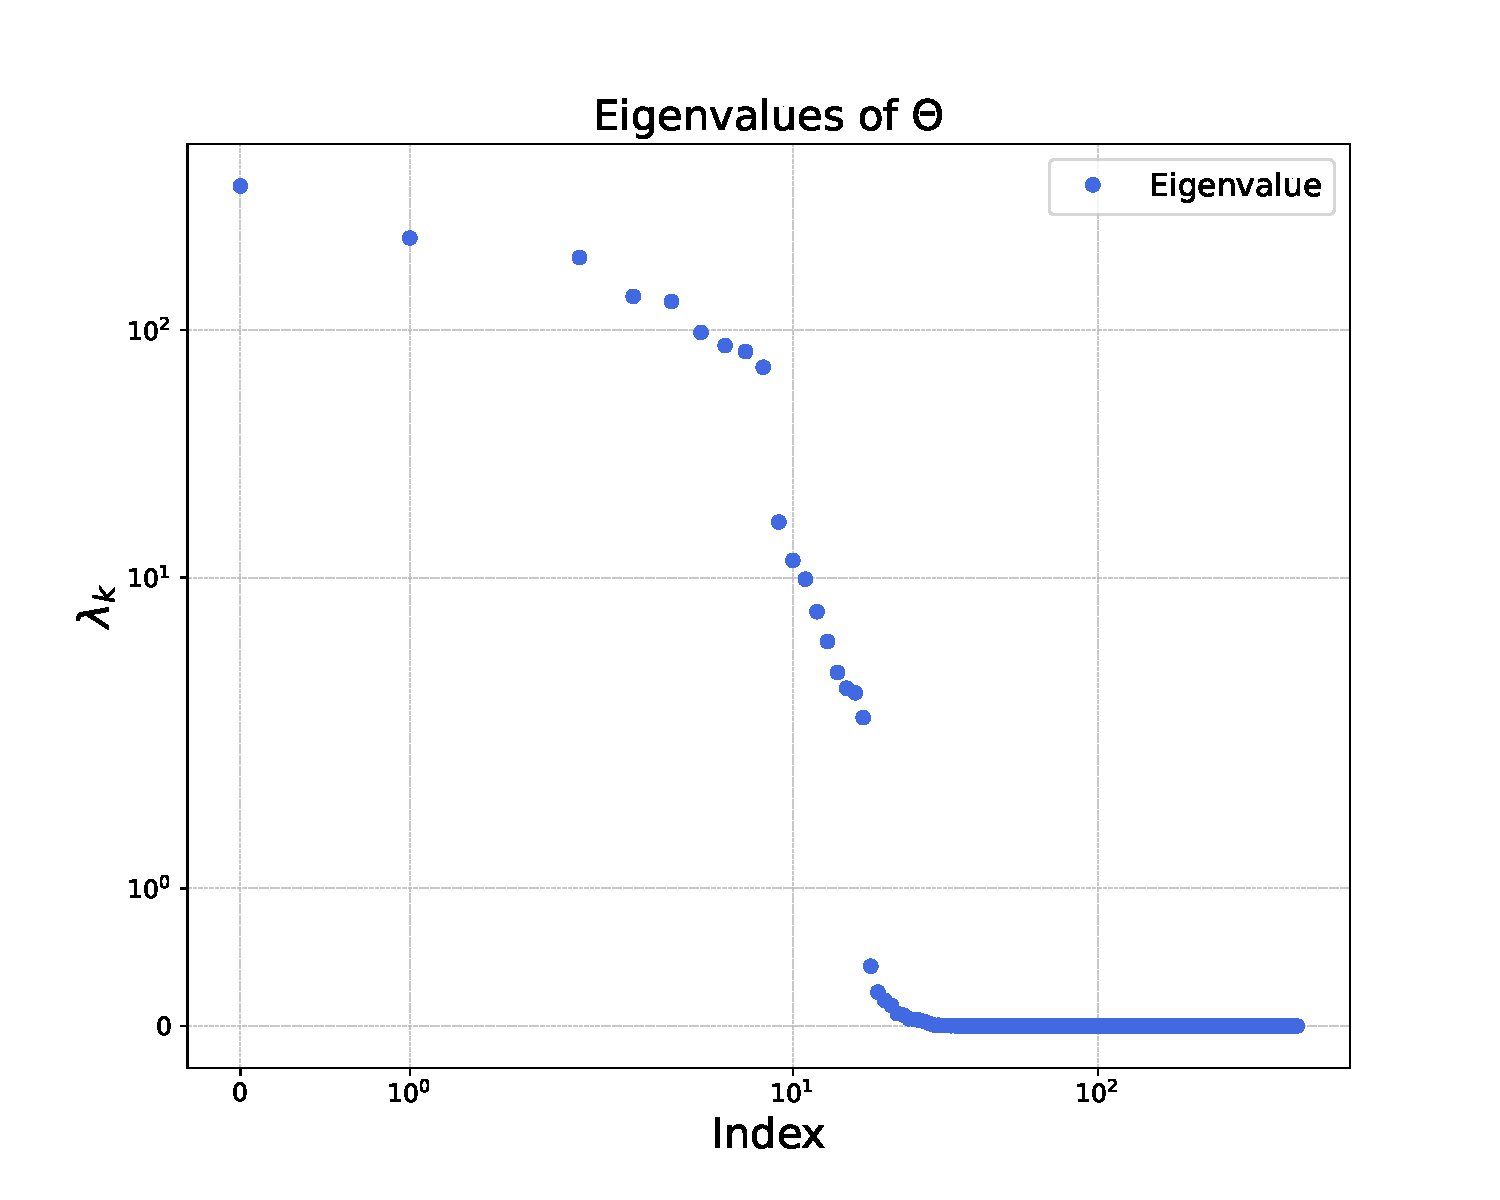
\includegraphics[width=0.4\textwidth]{ntk_eigvals.pdf}
  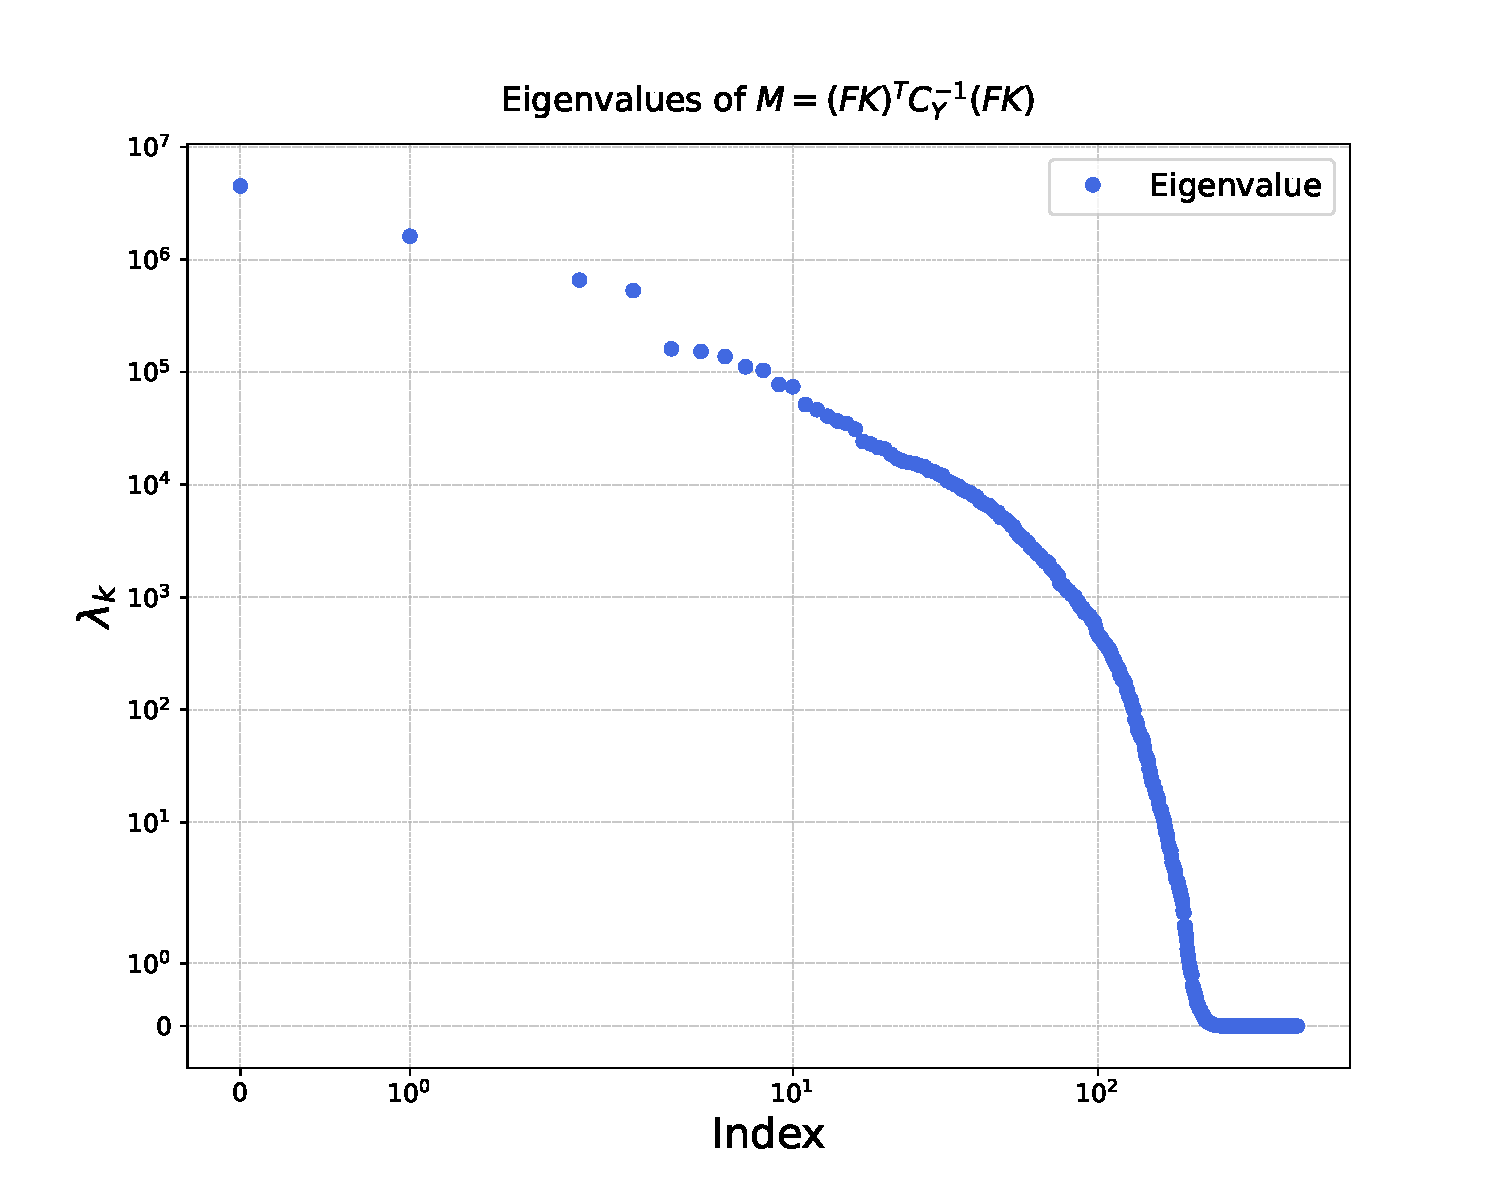
\includegraphics[width=0.4\textwidth]{m_eigvals.pdf}
  \caption{Eigenvalues of the NTK (left)
    and of the matrix $M$ (right) in logarithmic scale.}
  \label{fig:NTKEigVals}
\end{figure}
%%%%%%%%%%%%%%%%%%%%%%%%%%
The eigenvalues of the NTK, together with those of the matrix $M$, are displayed in
Fig.~\ref{fig:NTKEigVals}. We rewrite the flow equation, Eq.~\ref{eq:FlowLinearDataNTK}, as
\begin{align}
    \label{eq:ft_b_ThetaMft}
    \frac{d}{dt} f_t = b - \Theta M f_t\, , 
\end{align}
where 
\begin{align}
    \label{eq:Defb}
    b = \Theta \FKtabT C_Y^{-1} y\, ,
\end{align}
while the matrix $M$ has been introduced above.  Using the eigendecomposition $M = R D R^T$, 
where $R$ is an orthogonal matrix, we introduce 
\begin{align}
    \label{eq:RotatedF}
    \tilde{f}_t = D^{1/2} R^T f_t\, , \quad \tilde{b} = D^{1/2} R^T b\, ,
\end{align}
so that 
\begin{align}
    \label{eq:EvolutionRotatedF}
    \frac{d}{dt} \tilde{f}_t &= \tilde{b} - D^{1/2} R^T \Theta R D^{1/2} \tilde{f}_t \\
        &= \tilde{b} - \tilde{H} \tilde{f}_t\, .
\end{align}
The eigenvalues of the matrix $\tilde{H}$ are shown in Fig.~\ref{fig:Hevals}.
\begin{figure}[!ht]
    \centering
    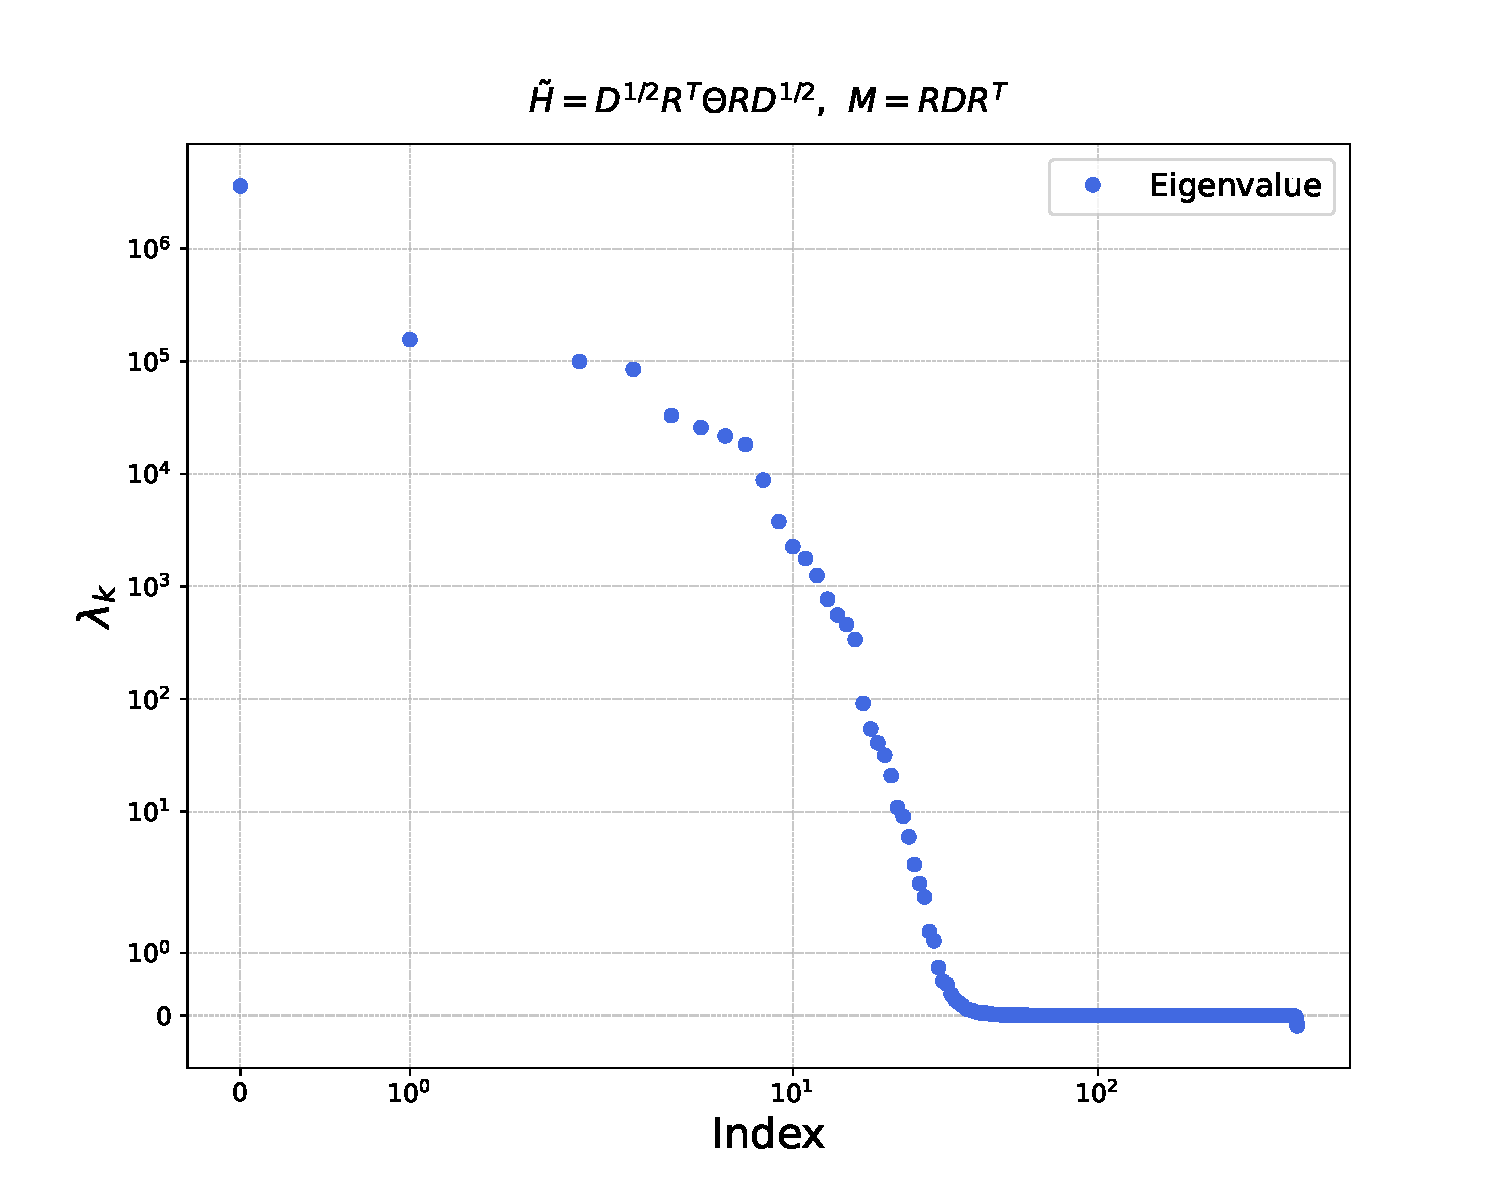
\includegraphics[width=0.6\textwidth]{Htilde_eigvals.pdf}
    \caption{Eigenvalues of $\tilde{H}$  
      in logarithmic scale.}
    \label{fig:Hevals}
  \end{figure}

\noindent
The solution, assuming that $\tilde{H}$ is independent of the flow time, is
\begin{align}
    \label{eq:FlowSolutionInFtilde}
    \tilde{f}_t = e^{-\tilde{H}t} \tilde{f}_0 + 
        \left(1 - e^{-\tilde{H}t}\right) \tilde{H}^{-1} \tilde{b}\, .
\end{align}
Taking the limit $t\to\infty$, we find
\begin{align}
    \label{eq:InfiniteTrainingF}
    f_\infty = M^{-1} \FKtabT C_Y^{-1} y = f^*\, ,
\end{align}
and thus
\begin{align}
    \label{eq:epsinfty}
    \epsilon_\infty = \left[
        1 - \FKtab M^{-1} \FKtabT C_Y^{-1} 
    \right] y\, .
\end{align}
A few lines of algebra yield
\begin{align}
    \frac12 ||\epsilon_\infty||_{C_Y}^2 = \mathcal{L}^*\, ,
\end{align}
in agreement with Eq.~\ref{eq:MinimumLossInf}. As before, if we consider a level-0 test, 
\begin{align}
    f_\infty = M^{-1} \FKtabT C_Y^{-1} \FKtab f^{\mathrm{in}} = f^{\mathrm{in}}\, .
\end{align}

\paragraph{Evolution for $\epsilon_t$.}
We can rewrite Eq.~\ref{eq:FlowLinearDataNTK} as 
\begin{align}
    \label{eq:FlowLinearDataNTKEpsilon}
    \frac{d}{dt} \epsilon_t &= - \FKtab \frac{d}{dt} f_t \nonumber \\
        &= - \FKtab \Theta \FKtabT C_Y^{-1} \epsilon_t \nonumber \\
        &= - \FKtab \Theta \FKtabT R_Y D_Y R_Y^T \epsilon_t\, ,
\end{align}
where we decompose $C_Y^{-1}=R_Y D_Y R_Y^T$.
Following the derivation for $f_t$, we define
\begin{align}
    \label{eq:RotatedEps}
    \tilde{\epsilon}_t = D_Y^{1/2} R_Y^T \epsilon_t\, , 
\end{align}
so that 
\begin{align}
     \frac{d}{dt} \tilde{\epsilon}_t = 
        - \tilde{H}_\epsilon \tilde{\epsilon_t}\, ,
\end{align}
where 
\begin{align}
    \label{eq:HSymmetricDef}
    \tilde{H}_\epsilon  = D_Y^{1/2} R_Y^T \FKtab \Theta \FKtabT R_Y D_Y^{1/2}
\end{align}
is a symmetric, positive definite, matrix, and therefore
\begin{align}
    \label{eq:SolutionForEpsilon}
    \epsilon_t = R_Y D_Y^{-1/2} e^{-\tilde{H}_\epsilon t} D_Y^{1/2} R_Y^T \epsilon_0\, .
\end{align}
Note that 
\begin{align}
    & \tilde{H}_\epsilon \tilde{\epsilon}_\infty = 
        D_Y^{1/2} R_Y^T \FKtab \Theta 
        \underbrace{\FKtabT C_Y^{-1}
        \left[
            1 - \FKtab M^{-1} \FKtabT C_Y^{-1}
        \right]}_{(*)} y\, , \nonumber \\
    & (*) = \FKtabT C_Y^{-1} - \underbrace{\FKtabT C_Y^{-1} \FKtab M^{-1}}_{= 1!} 
        \FKtabT C_Y^{-1} = 0\, ,
    \label{eq:EpsilonZeroMode}
\end{align}
and therefore the evolution operator for $\tilde{\epsilon}$, $\tilde{H}_\epsilon$, has a zero mode, which is 
not driven to zero by the gradient flow. The zero mode is exactly $\epsilon_\infty$, \ie\ the residual error 
at the end of the gradient flow. All other components of $\epsilon_t$ vanish exponentially with $t$.
This result is consistent with the result above for the evolution of $f_t$. Now we need to 
check them numerically! 

\paragraph{Consistency of the two evolutions.}
As a cross check of our calculation, we verify that the evolution of 
$\epsilon_t$ is consistent with the evolution of $f_t$. Starting from Eq.~\ref{eq:RotatedEps}, 
\begin{align}
    \label{eq:RotEpsRotF}
    \tilde\epsilon_t = D_Y^{1/2} R_Y^T 
        \left(y - \FKtab R D^{-1/2} \tilde{f}_t\right)\, . 
\end{align}
We compute separately the time-independent and the time-dependent contributions to $\tilde\epsilon_t$ 
in the RHS of Eq.~\ref{eq:RotEpsRotF}. 
Starting from the time-independent terms, we have
\begin{align}
    y &- \FKtab R D^{-1/2} \tilde{H}^{-1} \tilde{b} = \nonumber \\ 
    &= y - \FKtab \underbrace{R D^{-1/2} \left[D^{-1/2} R^T\right.}_{=M^{-1}} \left. \Theta^{-1} \right. \underbrace{\left.R D^{-1/2}\right] 
        \left[D^{1/2} R^T\right.}_{=1} \left. \Theta \FKtabT C_Y^{-1} y\right] \nonumber \\
    \label{eq:TimeIndepEpsCheck}
    &= \epsilon_\infty\, ,
\end{align}
and therefore
\begin{align}
    D_Y^{1/2} R_Y^T \left(
        y - \FKtab R D^{-1/2} \tilde{H}^{-1} \tilde{b}
    \right) = \tilde{\epsilon}_\infty\, .
\end{align}
The time-independent component of $\tilde{\epsilon}_t$ yields $\tilde{\epsilon}_\infty$, as expected. 
The time-dependent terms in $\FKtab R D^{-1/2} \tilde{f}_t$ are
\begin{align}
    \label{eq:TimeDependentContribEpsTilde}
    \FKtab R D^{-1/2} e^{-\tilde{H}t} \left(\tilde{H}^{-1} \tilde{b} - \tilde{f}_0\right)\, .
\end{align}
Focussing on the first term above, 
\begin{align}
    \FKtab &R D^{-1/2} e^{-\tilde{H}t} \tilde{H}^{-1} \tilde{b} = \nonumber \\
    & = \FKtab R D^{-1/2} \tilde{H}^{-1} \tilde{b} + \sum_{k>0} \FKtab R D^{-1/2} \frac{(-t)^k}{k!} \left(
        D^{1/2} R^T \Theta R D^{1/2}
    \right)^{k-1} D^{1/2} R^T b \nonumber \\
    & = \FKtab R D^{-1/2} \tilde{H}^{-1} \tilde{b} + \sum_{k>0} \frac{(-t)^k}{k!} \underbrace{\FKtab \left(\Theta M\right)^{k-1}}_{(*)} b\, .
\end{align}
Note that 
\begin{align}
    (*) &= \FKtab \underbrace{\left[\Theta \FKtabT C_Y^{-1} \FKtab\right] \left[\Theta \FKtabT C_Y^{-1} \FKtab\right] \ldots }_{k-1\ \mathrm{factors}} \\
    &= \underbrace{ \left[\FKtab \Theta \FKtabT C_Y^{-1}\right] \left[\FKtab\Theta \FKtabT C_Y^{-1}\right] \ldots }_{k-1\ \mathrm{factors}}  \FKtab\\
    &= \left[\FKtab \Theta \FKtabT C_Y^{-1}\right]^{k-1} \FKtab\, ,
\end{align}
and therefore 
\begin{align}
    \FKtab R D^{-1/2} e^{-\tilde{H}t} \tilde{H}^{-1} \tilde{b} = 
        \sum_k \frac{(-t)^k}{k!} \left[\FKtab \Theta \FKtabT C_Y^{-1}\right]^k y - \epsilon_\infty\, .
\end{align}
Hence the contribution to $\tilde{\epsilon}_t$ from this term
\begin{align}
    \sum_k & \frac{(-t)^k}{k!} D_Y^{1/2} R_Y^T \left[\FKtab \Theta \FKtabT R_Y D_Y^{1/2} D_Y^{1/2} R_Y^T\right]^k y = \nonumber \\
        &= \sum_k \frac{(-t)^k}{k!} \left[D_Y^{1/2} R_Y^T \FKtab \Theta \FKtabT R_Y D_Y^{1/2} \right]^k D_Y^{1/2} R_Y^T y \nonumber \\
        \label{eq:FirstTerm}
        &= e^{-\tilde{H}_\epsilon t} \left(\tilde{y} - \tilde{\epsilon}_\infty\right)\, .
\end{align}
The second term in Eq.~\ref{eq:TimeDependentContribEpsTilde} reads
\begin{align}
    \FKtab R D^{-1/2} e^{-\tilde{H}t} \tilde{f}_0 
        &= \FKtab R D^{-1/2} e^{-\tilde{H}t} D^{1/2} R^T f_0 \\
        &=  \sum_k \frac{(-t)^k}{k!} \FKtab \left(\Theta M\right)^k f_0 \\
        &= \sum_k \frac{(-t)^k}{k!} \left[\FKtab \Theta \FKtabT C_Y^{-1}\right]^k \FKtab f_0 \, ,
\end{align}
and hence the contribution to $\tilde{\epsilon}_t$
\begin{align}
    \label{eq:SecondTerm}
    D_Y^{1/2} R_Y^T R_Y D_Y^{-1/2} e^{-\tilde{H}_\epsilon t} D_Y^{1/2} R_Y^T \FKtab f_0
        = e^{-\tilde{H}_\epsilon t} D_Y^{1/2} R_Y^T \left(\FKtab f_0\right)\, .
\end{align}
Combining Eqs.~\ref{eq:FirstTerm} and~\ref{eq:SecondTerm} yields
\begin{align}
    \label{eq:TimeDepEpsCheck}
    e^{-\tilde{H}_\epsilon t} D_Y^{1/2} R_Y^T \left(y - \FKtab f_0\right) - \tilde{\epsilon}_\infty = 
    e^{-\tilde{H}_\epsilon t} \tilde{\epsilon}_0 - \tilde{\epsilon}_\infty\, .
\end{align}
And finally, adding Eqs.~\ref{eq:TimeIndepEpsCheck} and~\ref{eq:TimeDepEpsCheck}, we obtain
\begin{align}
    \label{eq:FinalResultEvolutionCheck}   
    \tilde{\epsilon}_t =  e^{-\tilde{H}_\epsilon t} \tilde{\epsilon}_0 \, ,
\end{align}
as expected.

% ------------------ Paragraph ----------------------
\subsection{Evolution of $f_t$ revisited.}
We start again from the eigenvectors and eigenvalues of $\Theta$
\begin{equation}
  \Theta \pmb{e}^{(k)} = \lambda_k \pmb{e}^{(k)}\,,
\end{equation}
to which we apply the same analysis carried out in Appendix~\ref{app:zero_mode}.
In this section, we use a feed-forward neural network with architecture
$[1,28,20,9]$. The activation function used in both the two deep layers is
\texttt{tanh}, while the output function is linear. The weights, rescaled by the
square root of the size of the previous layer, are initialised using a normal
distribution. The biases are initialised to zero. The input data are the points
of the grid in $x$-space taken from the FK tables.

We start by looking at the NTK matrix, displayed in the left panel of
Fig.~\ref{fig:NTKDecomposition}. Upon inspecting the figure, we see that the NTK
is uniform across flavours and bins in $x$. This is indeed expected, as the NTK
does not bring any physical information and it does not favour any particular
flavour to start with. In other words, the left plot in Fig.~\ref{fig:NTKDecomposition} 
shows the amount of information per flavour that we can ever reach given 
the network architecture and the choice of the grid in $x$.

The right panel of Fig.~\ref{fig:NTKDecomposition} shows the decomposition of
the NTK matrix in terms of the singular values and in terms of the eigenvalues.
The relative machine precision for double precision floating numbers ($\epsilon
\sim 2.2 \times 10^{-16}$) is also shown. We see that the singular values and
eigenvalues start to diverge when machine precision is reached. This is a
symptom of noise in the decomposition, and values below this threshold are set
to zero. Above threshold, the singular values and eigenvalues are consistent
and they show the usual hierarchy of the NTK extensively discussed in the
literature.
% Figure ----------------------
\begin{figure}[!t]
  \centering
  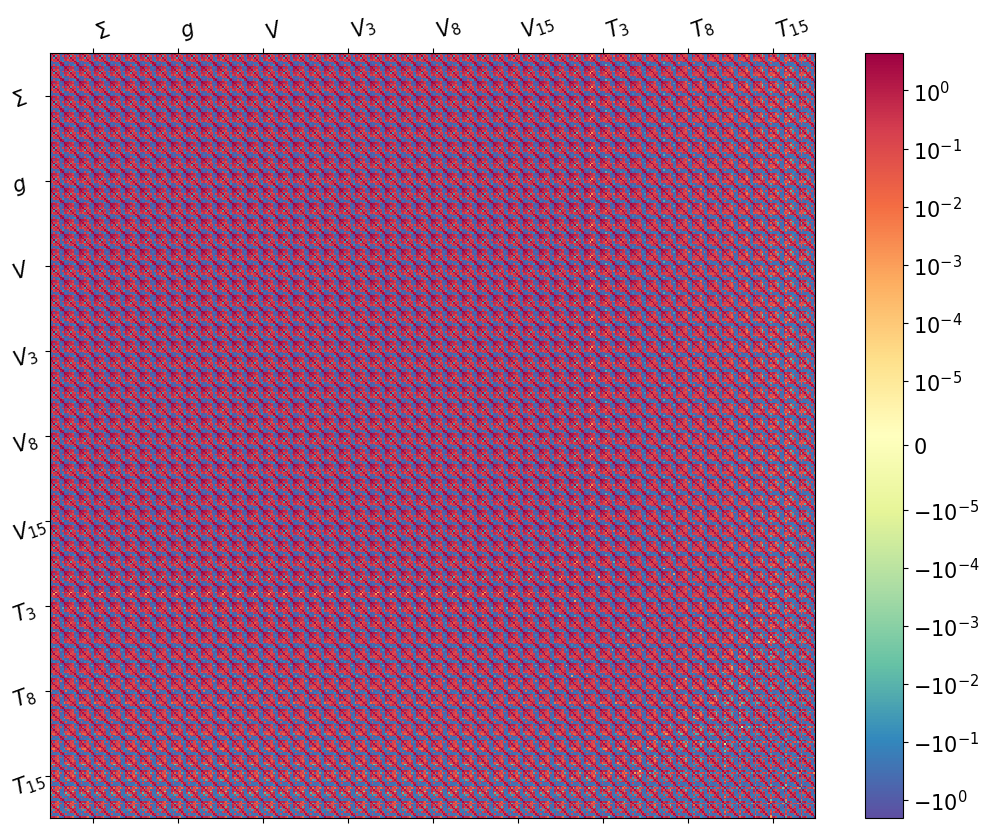
\includegraphics[width=0.4\textwidth]{ntk_matrix.png}
  \hspace{0.05\textwidth}
  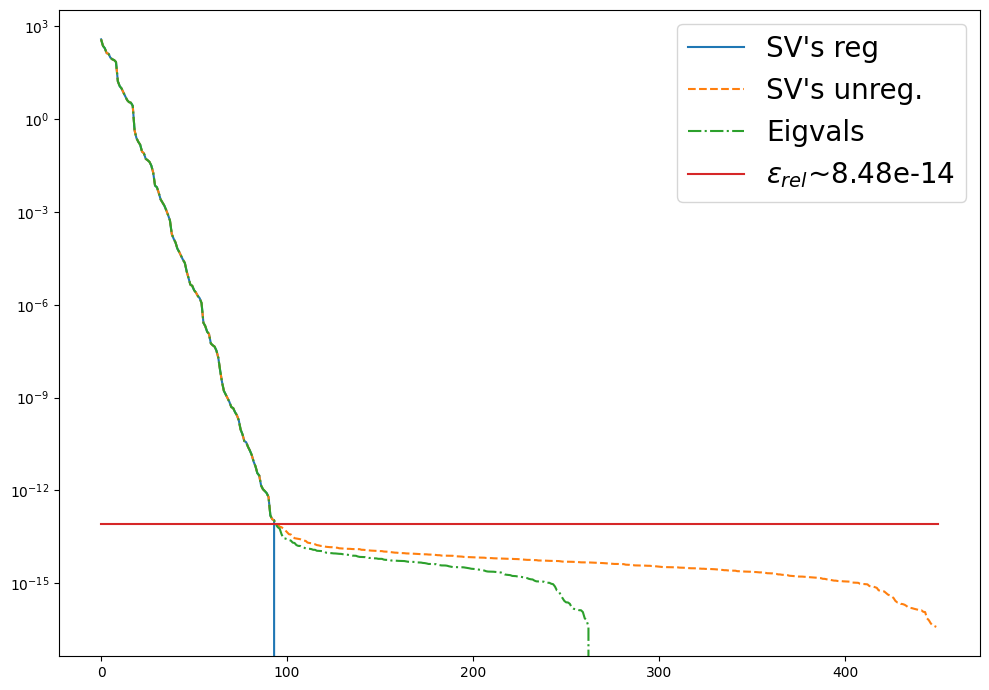
\includegraphics[width=0.4\textwidth, height=5cm]{ntk_decomposition.png}
  \caption{\small (Left) Representation of the NTK matrix in logarithmic scale. 
          (Right) Decomposition of the NTK matrix in terms of the eigenvalues and of the
          singular values of the matrix $M$, and the subsequent regularisation (see main text).}
  \label{fig:NTKDecomposition}
\end{figure}
% Figure ----------------------

The physical information is brought in by the FK tables, which combine with NTK
in the flow equation, reported below for convenience
\begin{equation}
  \frac{d}{dt}\pmb{f}_t = \pmb{b} - \Theta M \pmb{f}_t \,.
  \label{eq:FlowEquation}
\end{equation}
In a standard ML application of neural networks, the evolution kernel in
eq.~\ref{eq:FlowEquation} would be the NTK solely. On the other hand, in the
context of PDF fitting, we are interested in solving the inverse problem that
arise from the factorization theorem, and that is encoded in the matrix M. This
introduces additional complications, as the inverse problem is generally
ill-posed and the matrix M is not well-defined (see
Appendix~\ref{app:zero_mode}). Moreover, the product taking place in the second
term on the rhs of the equation above mixes the NTK and the FK spaces, making it
harder to disentangle the information brought in by the NTK and the FK tables
separately. 

The resulting evolution kernel is shown in Fig.~\ref{fig:EvKernel}.
Compared to the left panel of Fig.~\eqref{fig:NTKDecomposition}, the kernel
preserves the same underlying structure, yet modified by the action of the FK
tables. We also see that the overall architecture (network and FK tables) is not
sensitive to the low-$x$ region, while the mid- and large-$x$ region is more
sensitive.

Unfortunately, the evolution kernel is singular and cannot be inverted as it is,
preventing any attempt to integrate the flow equation eq.~\eqref{eq:FlowEquation}.
In order to proceed, we need to decompose the kernel in its various components and
discard the zero modes. This is the subject of the next section.

% Figure ----------------------
\begin{figure}[!t]
  \centering
  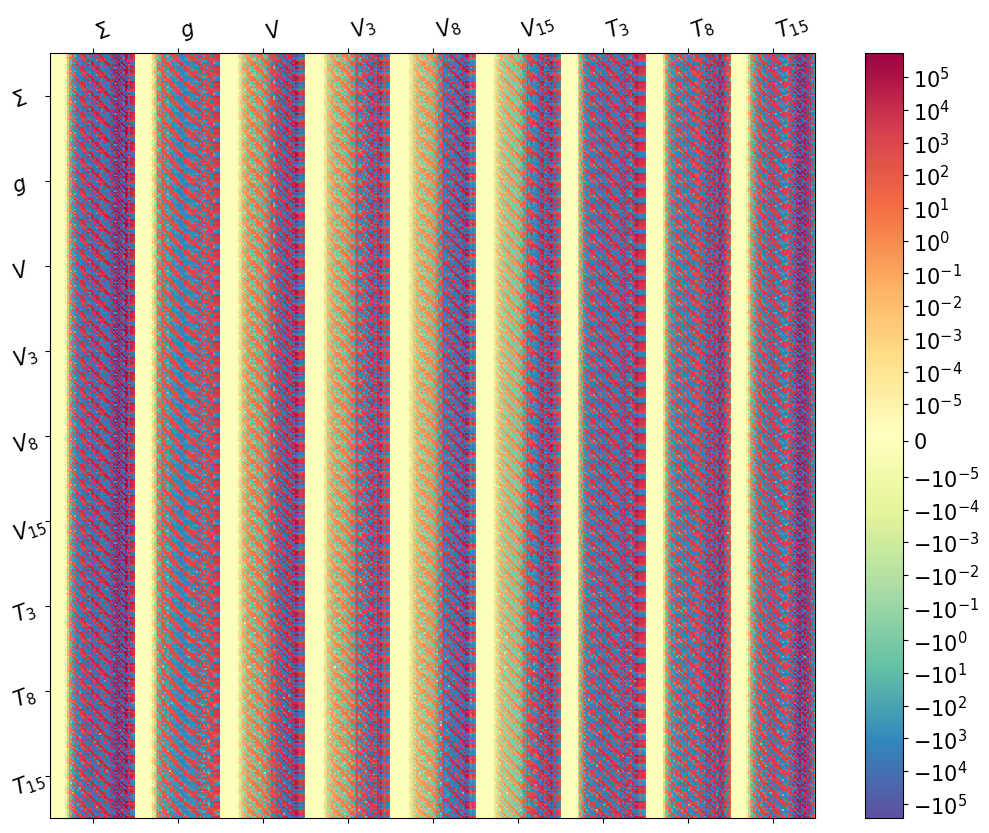
\includegraphics[width=0.8\textwidth]{evolution_kernel.png}
  \caption{\small}
  \label{fig:EvKernel}
\end{figure}
% Figure ----------------------

\subsubsection*{Projection of the flow equation}
The evolution kernel cannot be inverted directly, due to the presence of many zero
modes. We then resort to working in a subspace of the kernel, where it can be inverted.
In doing so, we will also try to disentangle the effects of the NTK and of the FK tables.

We start by projecting the flow equation in the eigenspace of the NTK, so that
we have
\begin{equation}
  \frac{d}{dt}f_{k,t}' = b_k' - \lambda_k (\pmb{e}^{(k)}, M \pmb{f}_t).
  \label{eq:FlowEqNTKProjection}
\end{equation}
Here the prime denotes the $k$-th component of the vector in the eigenspace of
the NTK, and $(\pmb{e}^{(k)}, M f_t)$ is the ordinary scalar product. Eq.~\eqref{eq:FlowEqNTKProjection}
can also be recast into matrix form. Writing $\Theta = U_{\Theta} \Sigma_{\Theta} U_{\Theta}^T$, then
we have
\begin{equation}
  \frac{d}{dt}\pmb{f}_{t}' = \pmb{b}' - \Sigma_{\Theta} U_{\Theta}^T M U_{\Theta} \pmb{f}'
  = \pmb{b}' - \Sigma_{\Theta} M' \pmb{f}'.
  \label{eq:FlowEqNTKProjectionMatrix}
\end{equation}
The equation above
requires two observations. The first one is that some eigenvalues of the NTK are
actually zero, so that the second term on the rhs of
eq.~\eqref{eq:FlowEqNTKProjection} is zero. Furthermore, for the first term on
the rhs we have
\begin{equation}
  b_k' = (\pmb{e}^{(k)}, \pmb{b}) = (\pmb{e}^{(k)}, \Theta (FK)^T C_Y^{-1} \pmb{Y}) = 0 \hspace{5mm} \forall \pmb{e}^{(k)} \in Ker(\Theta) .
\end{equation}
Thus, for zero eigenvalues of the NTK, we have
\begin{equation}
  \frac{d}{dt} f_{k,t}' = 0 \hspace{5mm} \Rightarrow f_{k,t}' = f_{k,0}' ,
\end{equation}
abd this result holds regardless of the FK tables.

The second observation involves the matrix $M$. In particular, we can decompose
$M$ as follows
\begin{equation}
  M = LL^T = (RD^{1/2})(D^{1/2}R^T),
\end{equation}
where $D$ is the diagonal matrix of the eigenvalues (or singular values) of $M$
and $R$ is the matrix of the eigenvectors. Using the completness relation of the
vectors $\pmb{e}^{(k)}$, we can write
\begin{equation}
  M_{k_1 k_2}' = (e^{(k_1)}, L e^{(k)})(e^{(k)}, L^T e^{(k_2)}) = L_{k_1k}' (L^T)_{kk_2}' = L_{k_1k}' L_{k_2k}',
  \label{eq:MProjNTK}
\end{equation}
or, in matrix form,
\begin{equation}
  M' = U_{\Theta}^T M U_{\Theta} = U_{\Theta}^T L U_{\Theta} U_{\Theta}^T L^T U_{\Theta} = L' (L')^T ,
  \label{eq:MProjNTKMatrix}
\end{equation}
where in the second equality we have used the completeness relation of the eigenvectors.

A close-up inspection of $L'$ reveals that
\begin{equation}
  \begin{split}
    L_{k_1k_2}' & \equiv \left( \pmb{e}^{(k)}, RD^{1/2} \pmb{e}^{(k)} \right) \\
    & = e^{(k_1)}_{i_1} R_{i_1 i_2} \mu_{i_2} e_{i_2}^{(k_2)} \\
    & = e^{(k_1)}_{i_1} v^{(i_2)}_{i_1} \mu_{i_2} e_{i_2}^{(k_2)} \\
    & = \mu_{i_2} e_{i_2}^{(k_2)} (\pmb{e}^{(k_1)}, \pmb{v}^{(i_2)}),
  \end{split}
\end{equation}
which means that the intersection between the NTK and the FK tables takes place in the
scalar product of the last equality above.

By means of eq.~\eqref{eq:MProjNTK}, we can rewrite the flow equation as follows
\begin{equation}
  \frac{d}{dt}f_{k_1,t}' = b_{k_1}' - \lambda_{k_1} L_{k_1 k_2}' L_{k_3 k_2}' f_{k_3,t}' \,.
\end{equation}
Finally, in order to obtain a symmetric kernel, we can multiply both sides by $(L')^T$ so that we have
\begin{equation}
  \frac{d}{dt} \tilde{f}_{k_1,t}' = \tilde{b}_{k_1}' - \tilde{K}_{k_1 k_2} \tilde{f}_{k_2,t}'
  \label{eq:FlowEqSymmetricKernel}
\end{equation}
where $\tilde{f}_{k_1,t}'$ and $\tilde{b}_{k_1}'$ are the components rotated by the action of of
$L'$, and $\tilde{K}_{k_1 k_2}$ is the symmetric kernel defined as
\begin{equation}
  \tilde{K} = (L')^T \Sigma_{\Theta} L' .
  \label{eq:SymmetricKernel}
\end{equation}

\subsubsection*{Removing zero modes of the NTK}
In obtaining Eq.~\eqref{eq:FlowEqSymmetricKernel}, we have kept all the zero modes of the NTK.
However, we can filter them out and write an expression that contains zero modes of the FK tables
solely. To do so, we restart from eq.~\eqref{eq:FlowEqNTKProjectionMatrix}, and we recall that the
rotations applied to the vectors are
\begin{equation}
  \pmb{b}' = U_{\Theta}^T \pmb{b} \quad \text{and} \quad \pmb{f}_t' = U_{\Theta}^T \pmb{f}_t\,.
\end{equation}
In order to separate that zero modes, we can split the
vector $\pmb{f_t'}$ into a part that is orthogonal to the kernel of the NTK, and another
which lives in the kernel and hence is constant
\begin{equation}
  \frac{d}{dt} 
  \left(
    \begin{matrix}
      \pmb{f}_{\perp,t}' \\
      \pmb{f}_{\parallel,t}'
    \end{matrix}
  \right)
  =
  \left(
    \begin{matrix}
      \pmb{b}_{\perp}' \\
      \pmb{b}_{\parallel}'
    \end{matrix}
  \right)
  -
  \left(
    \begin{matrix}
      \Sigma_{\Theta} & 0 \\
      0 & 0
    \end{matrix}
  \right)
  \left(
    \begin{matrix}
      M_{\bot\bot}' & M_{\bot \parallel}' \\
      M_{\parallel\bot}' & M_{\parallel \parallel}' \\
    \end{matrix}
  \right)
  \left(
    \begin{matrix}
      \pmb{f}_{\perp,t}' \\
      \pmb{f}_{\parallel,t}'
    \end{matrix}
  \right)
\end{equation}
where the subscripts $\perp$ and $\parallel$ denote the components orthogonal
and parallel to the kernel of the NTK, respectively. The equation above unravels
as follows
\begin{align}
  & \frac{d}{dt} \pmb{f}_{\perp,t}' = \pmb{b}_{\perp}' - 
    \Sigma_{\Theta} \left( M_{\perp \perp}' \pmb{f}_{\perp,t}' + 
    M_{\perp \parallel}' \pmb{f}_{\parallel,t}' \right),\\[5pt]
  & \frac{d}{dt} \pmb{f}_{\parallel,t}' = \pmb{0} ,
\end{align}
where the second equation is a consequence of the fact that the kernel of the
NTK is a zero mode for the learning flow. Note that the parallel component
$\pmb{f}_{\parallel,t}'$ appears in the flow equation of $\pmb{f}_{\perp,t}'$,
but it does not evolve in time. Hence, it can be reabsorbed in the constant
factor $\pmb{b}_{\perp}'$, giving
\begin{equation}
  \frac{d}{dt} \pmb{f}_{\perp,t}' = \pmb{B}_{\perp}' - 
  \Sigma_{\Theta} M_{\perp \perp}' \pmb{f}_{\perp,t}',
  \label{eq:FlowEqNTKPerp}
\end{equation}
where
\begin{equation}
  \pmb{B}_{\perp}' = \pmb{b}_{\perp}' - \Sigma_{\Theta} M_{\perp \parallel}' \pmb{f}_{\parallel,t}'.
\end{equation}
Eq.~\eqref{eq:FlowEqNTKPerp} restricts the evolution of the vector $\pmb{f}_t'$
to the components orthogonal to the kernel of the NTK. The only flat directions
left are those encoded in the FK tables.

\subsubsection*{Flat directions of the FK tables}
Following the same reasoning that led to eq.~\eqref{eq:FlowEqSymmetricKernel}, we can
rewrite eq.~\eqref{eq:FlowEqNTKPerp} as follows
\begin{equation}
  \frac{d}{dt} \tilde{\pmb{f}}_{\perp,t}' = \tilde{\pmb{B}}_{\perp}' - \tilde{K}_{\perp} \tilde{\pmb{f}}_{\perp,t}',
  \label{eq:FlowEqSymmetricKernelPerp}
\end{equation}
where
\begin{equation}
  M_{\perp \perp}' = L_{\perp}' (L_{\perp}')^T, \quad
  \tilde{\pmb{f}}_{\perp,t}' = (L_{\perp}')^T \pmb{f}_{\perp,t}', \quad
  \text{and} \quad
  \tilde{K}_{\perp} = (L_{\perp}')^T \Sigma_{\Theta} L_{\perp}'.
\end{equation}

The entries of the symmetric kernel $\tilde{K}_{\perp}$ and its decomposition are shown
in the left and right panel of Fig.~... As previously done for then NTK, we can rewrite
this kernel as follows
\begin{equation}
  \tilde{K}_{\perp} = U_{K} \Sigma_K U_{K}^T,
  \label{eq:SymmetricKernelDecomposition}
\end{equation}
and rotate equation eq.~\eqref{eq:FlowEqSymmetricKernelPerp} to the eigenbasis of the kernel
\begin{equation}
  \frac{d}{dt} \hat{\pmb{f}}_{\perp} = \hat{\pmb{B}}_{\perp} - \Sigma_K \hat{\pmb{f}}_{\perp, t},
\end{equation}
where
\begin{equation}
  \hat{\pmb{f}}_{\perp} = U_{K}^T \tilde{\pmb{f}}'_{\perp}, \quad
  \text{and} \quad
  \hat{\pmb{B}}_{\perp} = U_{K}^T \tilde{\pmb{B}}'_{\perp}.
\end{equation}
As displayed in Fig.~..., the kernel contains many flat directions due to the FK tables. We can
then decompose the vectors as follows
\begin{equation}
  \frac{d}{dt} 
  \left(
    \begin{matrix}
      \hat{\pmb{f}}_{\perp \perp,t} \\
      \hat{\pmb{f}}_{\perp \parallel,t}
    \end{matrix}
  \right)
  =
  \left(
    \begin{matrix}
      \hat{\pmb{B}}_{\perp \perp} \\
      \hat{\pmb{B}}_{\perp \parallel}
    \end{matrix}
  \right)
  -
  \left(
    \begin{matrix}
      \Sigma_{K} & 0 \\
      0 & 0
    \end{matrix}
  \right)
  \left(
    \begin{matrix}
      \hat{\pmb{f}}_{\perp \perp,t} \\
      \hat{\pmb{f}}_{\perp \parallel,t}
    \end{matrix}
  \right)
\end{equation}
yielding the two independent equations
\begin{align}
  & \frac{d}{dt}\hat{\pmb{f}}_{\perp \perp,t} = 
  \hat{\pmb{B}}_{\perp \perp} - \Sigma_K \hat{\pmb{f}}_{\perp \perp,t} \\[5pt]
  & \frac{d}{dt}\hat{\pmb{f}}_{\perp \parallel,t} = 0.
\end{align}
Once inverted, the first equation provides the evolution of the components of the vector
orthogonal to the null space of both NTK and FK tables. To retrieve the original vector
in flavour basis, we need to apply to the solution for $\hat{\pmb{f}}_{\perp \perp,t}$
the inverse rotations applied so far. This gives
\begin{equation}
  \pmb{f}_t = \left[ U_{\Theta} \right]_{\perp} L_{\perp}' U_K \hat{\pmb{f}}_{\perp \perp,t},
\end{equation}
where $\left[ U_{\Theta} \right]_{\perp}$ is the subspace of the eigenvectors of the NTK that
is orthogonal to its kernel.

\subsubsection*{Properties of the symmetric kernel}
The kernel $\tilde{K}$ ...

% ------------------ End Paragraph ----------------------


\newpage
\subsection*{Obsolete Material -- to be deleted, later}

We then project the flow equation for $f_t$, Eq.~\ref{eq:FlowLinearDataNTK}, in this basis
\begin{align}
    \label{eq:FlowEigenbasisNTK}
    \frac{d}{dt} f_{i,t} = b_i - \lambda_i M_{ij} f_{j,t}\, ,
\end{align} 
where
\begin{align}
    f_{i,t} &= (v_i, f_t)\, , \\
    b_i &= (v_i, \Theta \FKtabT C_Y^{-1} y)\, \\
    M_{ij} &= (v_i, \FKtabT C_Y^{-1} \FKtab v_j)\, .
\end{align}
Note that $M$ is symmetric and positive definite. We can write $M = R D^{1/2} D^{1/2} R^T$ and repeat the 
derivation we did for the $\epsilon$.

To be continued... 

At order $O(1)$ in an expansion in $1/n$, where $n$ is the width of the NN, $\Theta$ is constant during training, and the flow equation can be integrated analytically, 
\begin{align}
    \label{eq:IntegrateFlowAtLeadingOrder}
    f_t = M^{-1}\, \FKtabT\, \left[
        \left(1 - e^{-\hat{\Theta}_Yt}\right) y +
        e^{-\hat{\Theta}_Y t} \FKtab f_0
    \right]\, .
\end{align}
where 
\begin{align}
    \label{eq:DefineThetaM}
    \Theta_Y &= \FKtabT \Theta\, \FKtab\, , \\
    \hat{\Theta}_Y &= \Theta_Y C_Y^{-1}\, , \\    
    M &=  \FKtabT \FKtab\, .
\end{align}
Note that, if $\FKtab$ were invertible, then for $t\to\infty$
\begin{align}
    \FKtab f_\infty = \FKtab M^{-1} \FKtabT y = y\, ,
\end{align}
and the theoretical predictions go exactly through the points. However this is not true in the real life scenario where $\FKtab$ is {\em not}\ invertible. It is therefore interesting to compute the matrix (in data space)
\begin{align}
    \FKtab M^{-1} \FKtabT \, ,    
\end{align}
in order to understand how close the training can get to the training points. 

For points $f^*$ that do not enter in the computation of the theory prediction, the flow 
equation is
\begin{align}
    \label{eq:FlowStarLinearDataNTK}
    \frac{d}{dt} f^*_t = 
        \Theta^*_t\, \FKtab^T C_Y^{-1} \epsilon_t\, ,
\end{align}
where 
\begin{align}
    \label{eq:NTKStarDef}
    \Theta^*_t = \sum_{\mu,\nu}\, \lambda_{\mu\nu} \left(\nabla_\mu f^*_t\right)\, 
    \left(\nabla_\nu f_t\right)^T\, .
\end{align}
The solution to this flow equation is
\begin{align}
    \label{eq:IntegrateFlowAtLeadingOrderStar}
    f^*_t = \Theta^*\, \Theta^{-1}\, f_t \, . 
\end{align}
Need to check the constant term so that the boundary condition at $t=0$ is correct. 


\bibliographystyle{plain}
\bibliography{ntk.bib}

\appendix
\section{Null space of FK}
The FK tables can be regarded as a linear map from the space of PDFs to the space of 
data:
\begin{align}
  \FKtab : \mathbb{R}^{\PDF} \rightarrow \mathbb{R}^{\ndat} \,.
\end{align}
Note that the matrix corresponding to this linear map is not square, and hence $\FKtab 
\neq \FKtabT$. We can define the null space of the FK tables
\begin{equation}
  \ker \FKtab \equiv K_{\FKtab} = 
  \left\{
    f \in \mathbb{R}^{\PDF} \; : \; \FKtab \, f = 0
  \right\} \, ,
  \label{eq:ker_FK}
\end{equation}
together with its orthogonal space
\begin{equation}
  R_{\FKtab} \equiv K_{\FKtab}^{\bot} = 
  \left\{
    f \in \mathbb{R}^{\PDF} \; : \; f \cdot f_K = 0,
    \hspace{2mm} \forall f_K \in K_{\FKtab}
  \right\}\,.
\end{equation}
Note that 
\begin{align}
  \label{eq:KerFK->KerM}
  \FKtab f = 0 \Longrightarrow M f = 0\, .
\end{align}
The converse is also true, 
\begin{align}
  M f = 0 &\Longrightarrow (f, Mf) = 0 \\
    &\Longrightarrow (\FKtab f, C_Y^{-1} \FKtab f) = 0 \\
    &\Longrightarrow \FKtab f = 0\, ,
\end{align}
where the last inequality follows from the fact that $C_Y>0$.

For each of these two subspaces we can define a basis
\begin{align}
  & \B_{K} = \left\{ \pmb{u}^{(i)}_{K}\,, \hspace{2mm}  i=1,\dots, \dim K_{\FKtab} \right\} \,,\\
  & \B_{\bot} = \left\{ \pmb{u}^{(i)}_{\bot}\,, \hspace{2mm}  i=1,\dots, \dim R_{\FKtab} \right\} \,.
  \label{eq:FK_basis}
\end{align}
Remember that $K_{\FKtab} \bigoplus R_{\FKtab} = \mathbb{R}^{\PDF}$ and thus the basis $\B = \B_{K}
\bigoplus \B_{\bot}$ is a basis for $\mathbb{R}^{\PDF}$. Henceforth, when decomposing a vector in $\RPDF$, I 
will use the ordering $\left\{ \B_{K}, \B_{\bot} \right\}$. Hence, given $\pmb{f}\in \RPDF$, we can
write
\begin{equation}
  \pmb{f} = \pmb{f}_{K} + \pmb{f}_{\bot} 
          = \bpmat 
              f_K \\[2pt]
              f_{\bot}
            \epmat \,.
\end{equation}
Finally, note that $\FKtab$ is not symmetric (not even square). Thus, the right null space is not the same
as the left null space, in particular
\begin{align}
  \FKtab \pmb{u}_K = 0  \; \nRightarrow \; \pmb{u}_K^T \FKtab = 0 \,.
\end{align}

With the two bases in eqs.~\eqref{eq:FK_basis}, we can decompose the $\FKtab$ as follows
\begin{equation}
  \FKtab =
  \bpmat
    \FKtab_{KK}     & \FKtab_{K\bot} \\[3pt]
    \FKtab_{\bot K} & \FKtab_{\bot\bot}
  \epmat \,,
\end{equation}
where
\begin{align}
  \FKtab_{B_1 B_2} = \sum_{i=1}^{\dim\B_1} \sum_{j=1}^{\dim\B_2}
  \bra{u_{\B_1}^{(i)}} M \ket{u_{\B_2}^{(j)}} \;
  \pmb{u}_{\B_1}^{(i)} \pmb{u}_{\B_2}^{(j)}\,,
  \hspace{5mm}
  \B_1, \B_2 = K_{\FKtab}, R_{\FKtab}\,.
\end{align}
By definition of the kernel, we also have
\begin{align}
  \FKtab_{KK} = \FKtab_{\bot K} = 0 \,,
\end{align}
while $\FKtab_{K\bot}$ would be zero only if $\FKtab$ was diagonal. Thus, in the basis
$\B$, the FK tables can be expressed as
\begin{align}
  \FKtab =
  \bpmat
    0  & \FKtab_{K\bot} \\[3pt]
    0 & \FKtab_{\bot\bot}
  \epmat \,.
\end{align}
The product with a vector $\pmb{f} \in \RPDF$ becomes
\begin{equation}
  \FKtab \pmb{f} =
    \bpmat
      0  & \FKtab_{K\bot} \\[3pt]
      0  & \FKtab_{\bot\bot}
    \epmat
    \bpmat 
      f_K \\[2pt]
      f_{\bot}
    \epmat
    = \biggl(\FKtab_{K\bot} + \FKtab_{\bot\bot}\biggr) f_{\bot} \,.
\end{equation}

What are the implications for the matrix $M$? ...
\section{Numerical validation of eq.~\eqref{eq:EpsilonZeroMode}}
\label{app:zero_mode}
In eq.~\eqref{eq:EpsilonZeroMode} we showed that the solution for
$\varepsilon_{\infty}$ in the limit of infinite training length corresponds to
the zero mode of the evolution matrix in data space $\tilde{H}_{\varepsilon}$.
Here we provide the numerical argument that supports this result.

We start from the matrix $M$ which, roughly speaking, is the contraction of two
FK tables. Since FK tables contain many zeros, the matrix $M$ will be sparse.
The matrix $M$ is displayed element-wise in Fig.~\ref{fig:MatrixM}. Each block
identifies a flavour, and the length of the side of the block is equal to the
size of the grid. 
% Figure ----------------------
\begin{figure}[h]
  \centering
  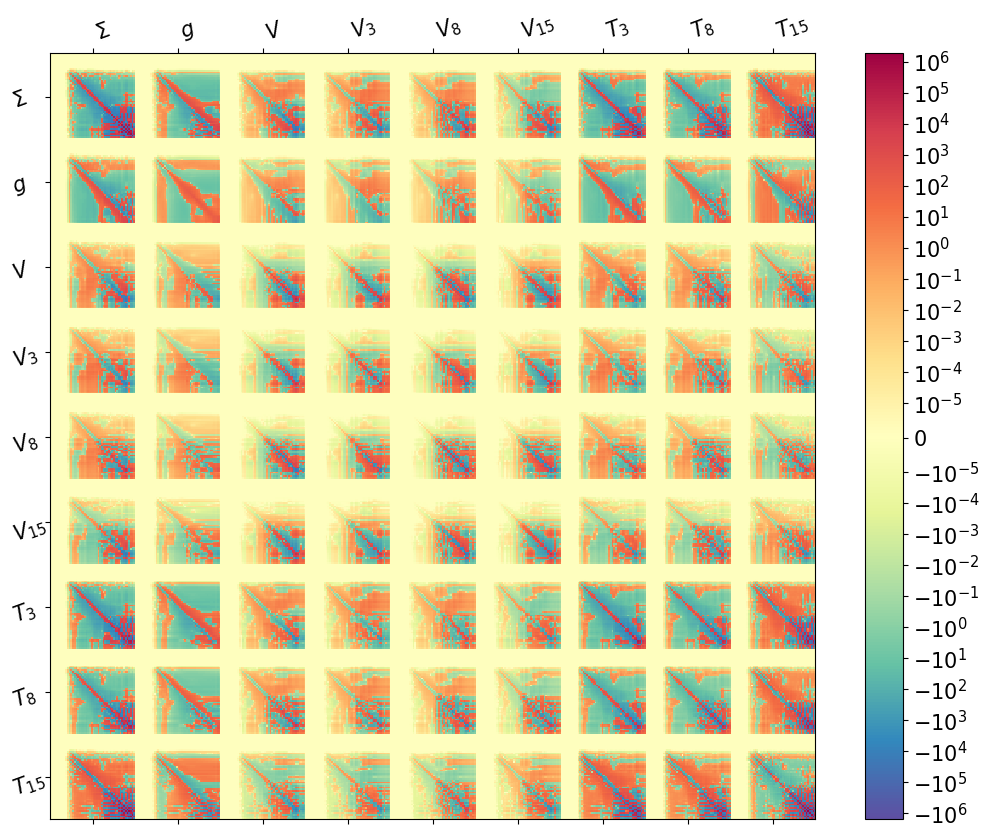
\includegraphics[width=0.5\textwidth]{M_matrix.png}
  \caption{\small Matrix $M$ in logarithmic scale.}
  \label{fig:MatrixM}
\end{figure}
%----------------------
The matrix $M$ is decomposed using the singular value decomposition (SVD) method
\begin{equation}
M = U \Sigma V^T \,,
\end{equation}
where $U$ and $V$ are orthogonal matrices, and $\Sigma$ is a diagonal matrix
containing the singular values sorted in decreasing order. Recall that the
matrix $M$ is also symmetric by construction, and this guarantees the existence
of the solution of the associated eigensystem. Singular values and the absolute
eigenvalues are displayed in Fig.~\ref{fig:eig_svd_M}. Here we also show the
relative machine precision error, defined as the product of the largest singular
value with the machine precision for double precision floating numbers
($\epsilon \sim 2.2 \times 10^{-16}$). Since the largest singular value is of
order $10^6$, the relative machine precision error is
$\epsilon_{\textrm{rel}}\sim1.2\times 10^{-9}$. The relevance of this number
will be clear in the following observation.

As it can be seen from the figure, the singular values and the eigenvalues
overlap as long as the relative numerical precision is not reached. Once this
numerical threshold is exceeded, the two sets of values start to diverge. This
is a consequence of the fact that $\epsilon_{\textrm{rel}}$ defines the smallest
double floating number that machine precision allows us to distinguish.
Everything below this value is noise and should be discarded. This prompts us to
apply an \textit{ad hoc} regularisation to $\Sigma$, whereby the values below
$\epsilon_{\textrm{rel}}$ are set to zero.
% Figure ----------------------
\begin{figure}[h]
  \centering
  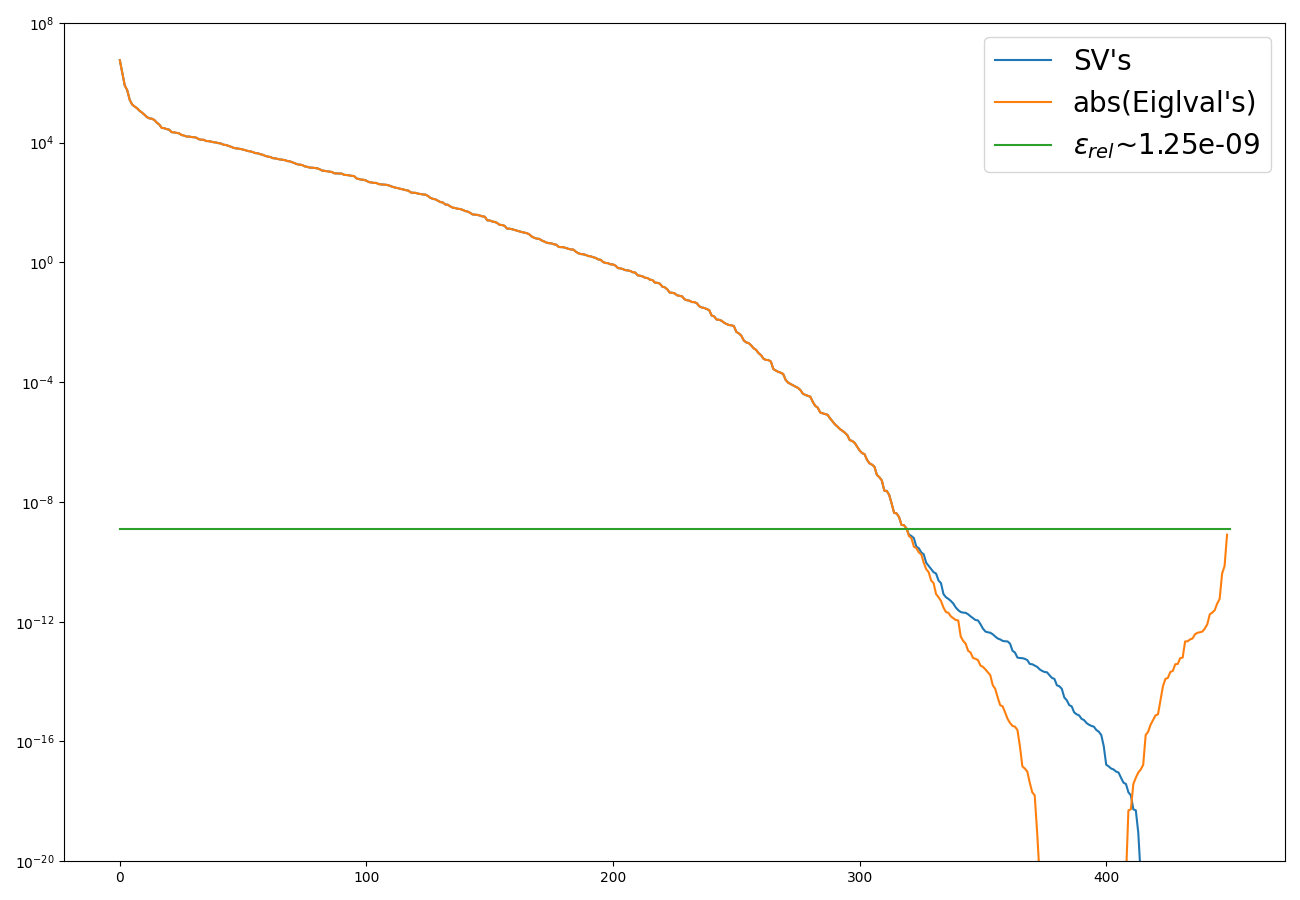
\includegraphics[width=0.5\textwidth]{eig_svd_M.png}
  \caption{\small Singular values and (absolute) eigenvalues of the matrix $M$
    plotted in logarithmic scale. The green horizontal line marks the relative
    machine precision error, as explained in the main text.}
  \label{fig:eig_svd_M}
\end{figure}
%----------------------
Note that we have also checked that the singular vectors of $U$ and $V$ are the
same if they are associated to the singular values above the numerical
threshold. In other words, in the space orthogonal to Ker$(M)$, the SVD matches
the eigendecomposition.

In principle, the singular vectors of the non-zero values span the space
orthogonal to Ker$(M)$. In this subspace, the matrix $M$ is diagonal and the
entries are exactly the non-zero singular values. However, if we compute the
condition number of $M$ in this subspace, we find that it is remarkably large,
$\kappa(M) \sim 10^{15}$. In other words, even in this subspace the matrix $M$
is ill-defined and cannot be inverted. The solution to this problem is to
further reduce the dimensionality of the orthogonal space, at the cost of
introducing some arbitrariness into the problem. Specifically, the final
solution will depend on the number of small singular values that we discard. For
example, the solution at infinity, eq.~\eqref{eq:InfiniteTrainingF}, will be
influenced by this cut-off, as shown in Fig.~\ref{fig:InfiniteTrainingFCuts}. In
this figure, eq.~\eqref{eq:InfiniteTrainingF} is first computed in the truncated
orthogonal space; then the result is transformed back to the original flavour
basis using the matrix $U$ restricted to the vectors that span the (reduced)
orthogonal space.
% Figure ----------------------
\begin{figure}[h]
  \centering
  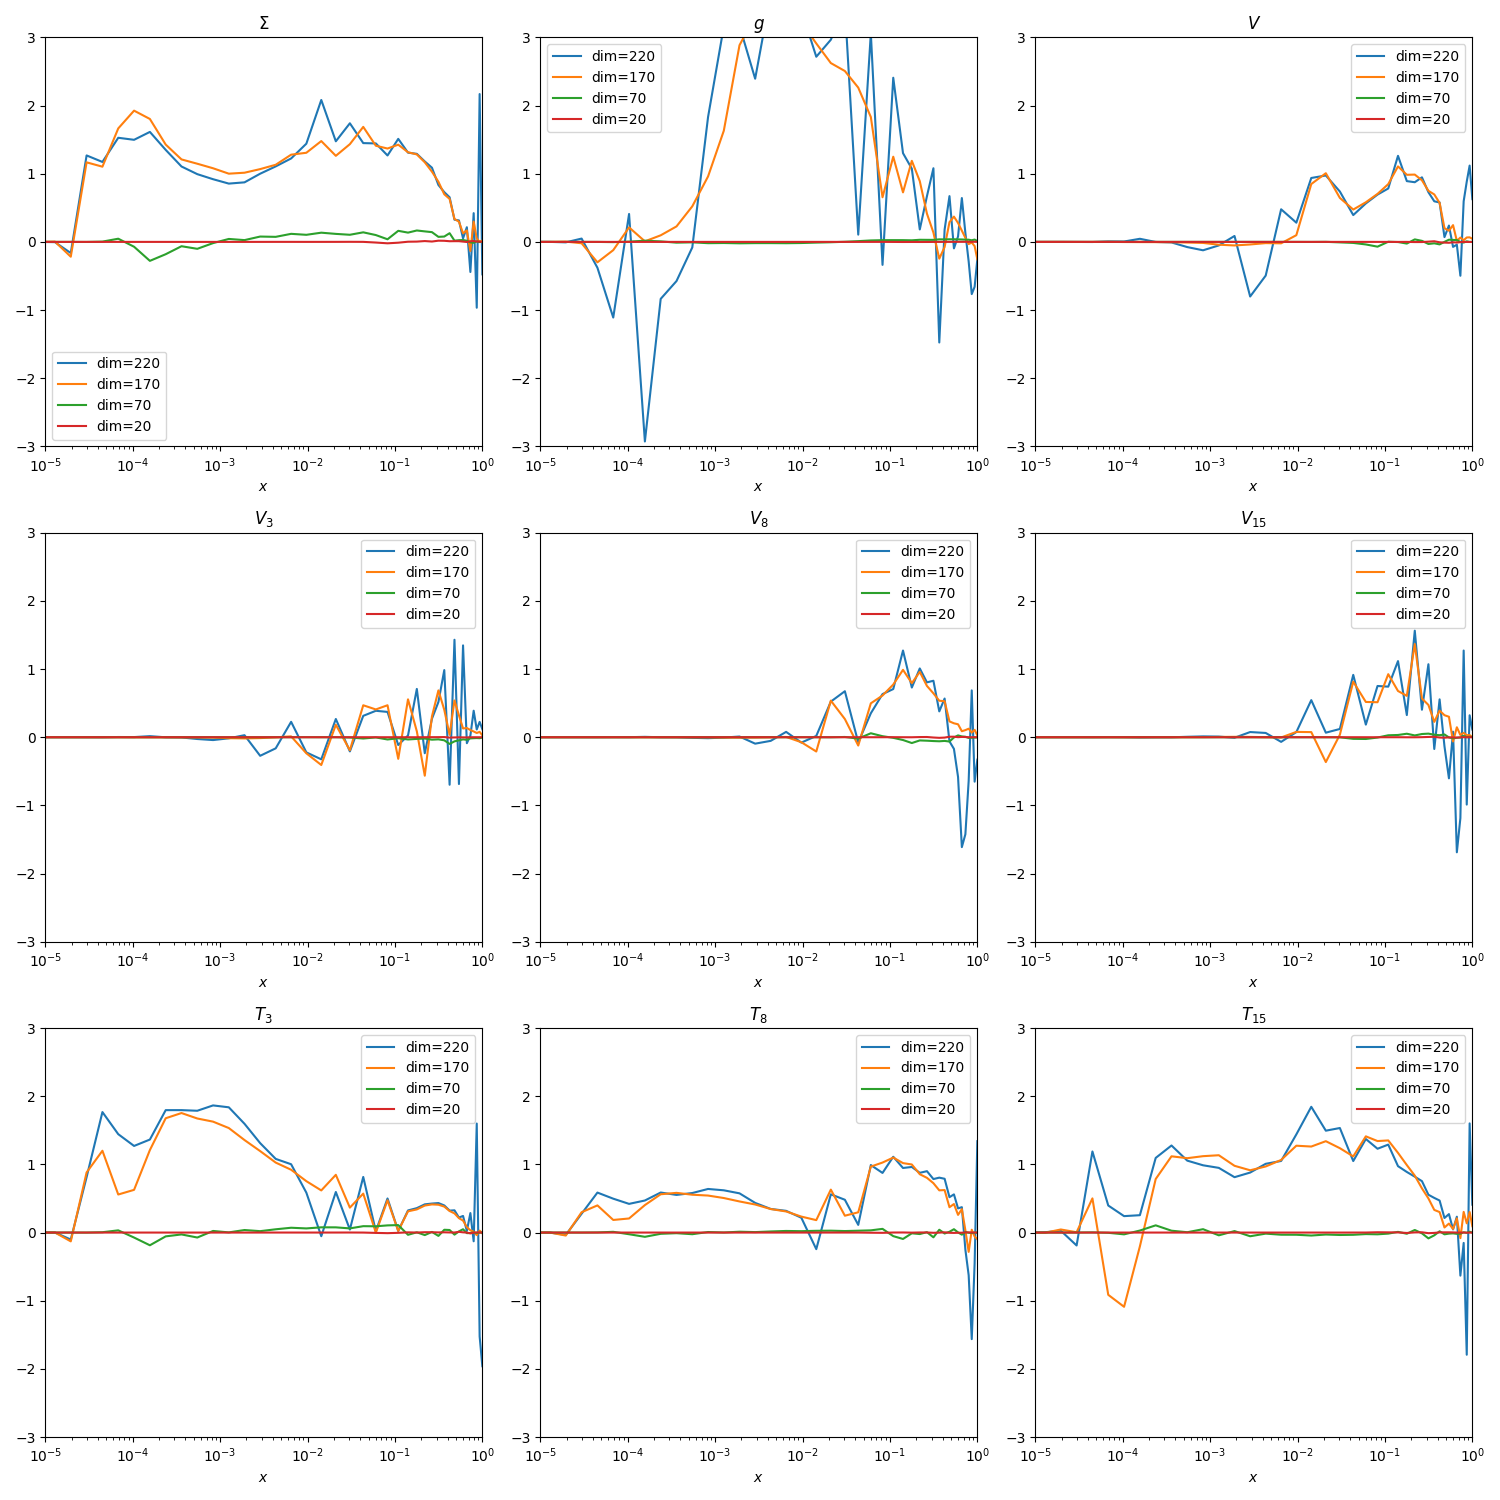
\includegraphics[width=0.7\textwidth]{f_inf.png}
  \caption{\small}
  \label{fig:InfiniteTrainingFCuts}
\end{figure}
%----------------------

As a final check, we can verify that eq.~\eqref{eq:EpsilonZeroMode} is
numerically satisfied. As we have just mentioned, even $\epsilon_{\infty}$ will depend
on the severity of the cut-off. We then expect different results as we modify the
number of singular values that we discard. For instance, using the orthogonal
subspace without any cut, eq.~\eqref{eq:EpsilonZeroMode} evaluates to
\begin{equation}
  \left| \tilde{H}_{\varepsilon} \varepsilon_{\infty} \right| \approx 0.28 \,.
\end{equation}
On the other hand, if we reduce the size of the subspace to $170$ (from 320), we
get
\begin{equation}
  \left| \tilde{H}_{\varepsilon} \varepsilon_{\infty} \right| \approx ~1.33 \times 10^{-5} \,.
\end{equation}



\end{document}

%%% Local Variables:
%%% mode: latex
%%% TeX-master: t
%%% End:
